\documentclass{article}

% content/resources/templates/preamble.tex
\usepackage[margin=0.6in]{geometry}
\author{Milav Dabgar}
\usepackage{amsmath,amssymb,amsthm}
\usepackage{booktabs}
\usepackage{multirow}
\usepackage{xcolor}
\usepackage{tcolorbox}
\tcbuselibrary{breakable,skins}
\usepackage[colorlinks=true,linkcolor=blue]{hyperref}
\usepackage{titlesec}
\usepackage{enumitem}
\usepackage{tikz}
\usepackage{pgfplots}
\usepackage{circuitikz}
\usepackage[version=4]{mhchem}
\usepackage{longtable}
\usepackage{array}
\usepackage{float}
\usepackage{caption}
\usepackage{listings}

\lstset{
  basicstyle=\small\ttfamily,
  breaklines=true,
  breakatwhitespace=false,
  postbreak=\mbox{\textcolor{red}{$\hookrightarrow$}\space},
  float=false,
  numbers=left,
  numberstyle=\tiny\color{gray},
  numbersep=10pt,
  xleftmargin=2em,
  keywordstyle=\color{blue},
  commentstyle=\color{green!60!black},
  stringstyle=\color{purple},
  backgroundcolor=\color{gray!5},
  showstringspaces=false,
  tabsize=2,
  captionpos=b,
  keepspaces=true,
  columns=flexible
}

\pgfplotsset{compat=1.18}
\usetikzlibrary{shapes,arrows,positioning,calc,patterns,decorations.pathmorphing,decorations.markings,arrows.meta}

% Color scheme
\definecolor{headcolor}{RGB}{0,102,204}
\definecolor{keycolor}{RGB}{220,20,60}
\definecolor{solutioncolor}{RGB}{34,139,34}
\definecolor{mnemoniccolor}{RGB}{148,0,211}
\definecolor{codecolor}{RGB}{0,0,100}

% Spacing
\setlength{\parskip}{3pt}
\setlist[itemize]{nosep}
\setlist[enumerate]{nosep}

% Title formatting
\titleformat{\section}{\Large\bfseries\color{headcolor}}{\thesection}{1em}{}
\titleformat{\subsection}{\large\bfseries\color{headcolor}}{\thesubsection}{1em}{}

% Pandoc tightlist compatibility
\providecommand{\tightlist}{%
  \setlength{\itemsep}{0pt}\setlength{\parskip}{0pt}}

% Pandoc longtable compatibility
\newcounter{none}
\def\thenone{}


% content/resources/templates/english-boxes.tex

% Custom environments
\newtcolorbox{solutionbox}{
 breakable,
 enhanced,
 colback=solutioncolor!5!white,
 colframe=solutioncolor!75!black,
 fonttitle=\bfseries,
 title=Solution
}

\newtcolorbox{solutionboxnobreak}{
 colback=solutioncolor!5!white,
 colframe=solutioncolor!75!black,
 fonttitle=\bfseries,
 title=Solution
}

\newtcolorbox{keyformula}{
 breakable,
 enhanced,
 colback=keycolor!5!white,
 colframe=keycolor!75!black,
 fonttitle=\bfseries,
 title=Key Formula
}

\newtcolorbox{mnemonicboxenv}{
 breakable,
 enhanced,
 colback=mnemoniccolor!5!white,
 colframe=mnemoniccolor!75!black,
 fonttitle=\bfseries,
 title=Mnemonic
}

\newcommand{\mnemonicbox}[1]{%
  \begin{mnemonicboxenv}
    #1
  \end{mnemonicboxenv}
}


% Custom commands for GTU solutions
% This file defines semantic commands for consistent formatting

% Question command with automatic formatting
\newcommand{\question}[2]{%
  \section*{Question #1}%
  \textbf{#2}%
}

% OR question variant
\newcommand{\questionor}[2]{%
  \section*{Question #1 OR}%
  \textbf{#2}%
}

% Proper table environment with caption
\newenvironment{answertable}[1]{%
  \begin{table}[htbp]
  \centering
  \caption{#1}
}{%
  \end{table}
}

% Proper figure environment for diagrams
\newenvironment{answerdiagram}[1]{%
  \begin{figure}[htbp]
  \centering
  \caption{#1}
}{%
  \end{figure}
}

% Semantic markup for key terms
\newcommand{\keyword}[1]{\textbf{#1}}
\newcommand{\code}[1]{\texttt{#1}}
\newcommand{\classname}[1]{\texttt{#1}}
\newcommand{\methodname}[1]{\texttt{#1}}

% Proper quotation marks
\newcommand{\mnemonic}[1]{``#1''}


\title{Linux Operating System (4331602) - Summer 2025 Solution}
\date{May 13, 2025}

\begin{document}
\maketitle

\questionmarks{1(a)}{3}{Define Operating System and explain the need of OS.}

\begin{solutionbox}
\textbf{Answer}:

\textbf{Operating System} is a system software that acts as an intermediary between computer hardware and application software. It manages hardware resources and provides services to user programs.

\textbf{Need of Operating System:}
\begin{itemize}
    \item \keyword{Resource Management}: Manages CPU, memory, storage, and I/O devices efficiently
    \item \keyword{User Interface}: Provides command-line and graphical interfaces for user interaction
    \item \keyword{Program Execution}: Loads and executes user programs safely
\end{itemize}
\end{solutionbox}

\begin{mnemonicbox}
\mnemonic{RUP - Resource, User, Program management}
\end{mnemonicbox}

\questionmarks{1(b)}{4}{Write a short note on Process Control Block (PCB).}

\begin{solutionbox}
\textbf{Answer}:

Process Control Block (PCB) is a data structure maintained by the operating system for each running process.

\begin{center}
\captionof{table}{PCB Components}
\begin{tabulary}{\linewidth}{|L|L|}
\hline
\textbf{PCB Component} & \textbf{Description} \\ \hline
Process ID & Unique identifier for the process \\ \hline
Process State & Current state (ready, running, waiting) \\ \hline
Program Counter & Address of next instruction to execute \\ \hline
CPU Registers & Values of CPU registers when process is suspended \\ \hline
Memory Management & Base and limit registers, page tables \\ \hline
I/O Status & List of open files and I/O devices \\ \hline
\end{tabulary}
\end{center}

\textbf{Key Functions:}
\begin{itemize}
    \item \keyword{Process Identification}: Stores unique process ID and parent process ID
    \item \keyword{State Information}: Maintains current execution state and context
    \item \keyword{Resource Allocation}: Tracks allocated resources and memory usage
\end{itemize}
\end{solutionbox}

\begin{mnemonicbox}
\mnemonic{PIS - Process ID, Information, State tracking}
\end{mnemonicbox}

\questionmarks{1(c)}{7}{List different types of Operating systems. Explain the working of batch operating systems with a suitable example.}

\begin{solutionbox}
\textbf{Answer}:

\textbf{Types of Operating Systems:}
\begin{center}
\captionof{table}{Types of Operating Systems}
\begin{tabulary}{\linewidth}{|L|L|}
\hline
\textbf{Type} & \textbf{Description} \\ \hline
Batch OS & Groups similar jobs and executes them together \\ \hline
Time-sharing OS & Multiple users share system simultaneously \\ \hline
Real-time OS & Provides guaranteed response time \\ \hline
Distributed OS & Manages multiple interconnected computers \\ \hline
Network OS & Provides network services and resource sharing \\ \hline
Mobile OS & Designed for mobile devices \\ \hline
\end{tabulary}
\end{center}

\textbf{Batch Operating System Working:}

\begin{center}
\begin{tikzpicture}[node distance=1.5cm, auto]
    \node [gtu block] (j1) {Job 1 \\ COBOL};
    \node [gtu block, right=0.5cm of j1] (j2) {Job 2 \\ FORTRAN};
    \node [gtu block, right=0.5cm of j2] (j3) {Job 3 \\ C++};
    \node [gtu block, right=0.5cm of j3] (j4) {Job 4 \\ JAVA};
    
    \node [gtu block, below=1.5cm of j2, xshift=1cm, minimum width=6cm] (manager) {Batch Queue Manager};
    
    \node [gtu block, below=1.5cm of manager, minimum width=2cm] (memory) {Memory \\ Manager};
    \node [gtu block, left=0.5cm of memory, minimum width=2cm] (cpu) {CPU \\ Executor};
    \node [gtu block, right=0.5cm of memory, minimum width=2cm] (io) {I/O \\ Handler};
    
    \draw [gtu arrow] (j1) -- (manager.north -| j1);
    \draw [gtu arrow] (j2) -- (manager.north -| j2);
    \draw [gtu arrow] (j3) -- (manager.north -| j3);
    \draw [gtu arrow] (j4) -- (manager.north -| j4);
    
    \draw [gtu arrow] (manager) -- (memory);
    \draw [gtu arrow] (memory) -- (cpu);
    \draw [gtu arrow] (memory) -- (io);
\end{tikzpicture}
\captionof{figure}{Batch Operating System}
\end{center}

\textbf{Example}: Bank transaction processing where all day's transactions are collected and processed together at night for efficiency.

\textbf{Key Features:}
\begin{itemize}
    \item \keyword{Job Grouping}: Similar jobs executed together for efficiency
    \item \keyword{No User Interaction}: Jobs run without user intervention once submitted
    \item \keyword{High Throughput}: Maximizes system utilization
\end{itemize}
\end{solutionbox}

\begin{mnemonicbox}
\mnemonic{JNH - Jobs grouped, No interaction, High throughput}
\end{mnemonicbox}

\questionmarks{1(c) OR}{7}{List different types of Operating systems. Explain the real time operating systems in detail.}

\begin{solutionbox}
\textbf{Answer}:

\textbf{Types of Operating Systems:}
(Same table as above)

\textbf{Real-Time Operating System (RTOS):}
Real-time OS provides guaranteed response within specified time constraints for critical applications.

\textbf{Types of RTOS:}
\begin{center}
\captionof{table}{Types of RTOS}
\begin{tabulary}{\linewidth}{|L|L|L|}
\hline
\textbf{Type} & \textbf{Deadline} & \textbf{Example} \\ \hline
Hard Real-time & Must meet deadline & Air traffic control, pacemaker \\ \hline
Soft Real-time & Can tolerate some delay & Video streaming, online gaming \\ \hline
Firm Real-time & Occasional deadline miss acceptable & Live audio processing \\ \hline
\end{tabulary}
\end{center}

\textbf{Characteristics:}
\begin{itemize}
    \item \keyword{Deterministic}: Predictable response time for all operations
    \item \keyword{Priority-based Scheduling}: High-priority tasks get immediate attention
    \item \keyword{Minimal Interrupt Latency}: Fast context switching capabilities
    \item \keyword{Memory Management}: Real-time memory allocation without delays
\end{itemize}

\textbf{Applications:}
\begin{itemize}
    \item Medical devices, automotive systems, industrial automation, aerospace control systems
\end{itemize}
\end{solutionbox}

\begin{mnemonicbox}
\mnemonic{DPMA - Deterministic, Priority-based, Minimal latency, Applications critical}
\end{mnemonicbox}

\questionmarks{2(a)}{3}{Differentiate between program and process.}

\begin{solutionbox}
\textbf{Answer}:

\begin{center}
\captionof{table}{Program vs Process}
\begin{tabulary}{\linewidth}{|L|L|L|}
\hline
\textbf{Aspect} & \textbf{Program} & \textbf{Process} \\ \hline
Definition & Static code stored on disk & Program in execution \\ \hline
State & Passive entity & Active entity \\ \hline
Memory & No memory allocation & Allocated memory space \\ \hline
Lifetime & Permanent until deleted & Temporary during execution \\ \hline
Resources & No resource consumption & Consumes CPU, memory, I/O \\ \hline
\end{tabulary}
\end{center}

\textbf{Key Differences:}
\begin{itemize}
    \item \keyword{Static vs Dynamic}: Program is static file, process is dynamic execution
    \item \keyword{Resource Usage}: Process consumes system resources, program doesn't
    \item \keyword{Multiple Instances}: One program can create multiple processes
\end{itemize}
\end{solutionbox}

\begin{mnemonicbox}
\mnemonic{SDR - Static vs Dynamic, Resource usage, Multiple instances}
\end{mnemonicbox}

\questionmarks{2(b)}{4}{Explain the different states of a process with the help of a process state diagram.}

\begin{solutionbox}
\textbf{Answer}:

\begin{center}
\begin{tikzpicture}[node distance=2cm, auto]
    \node [gtu state] (new) {New};
    \node [gtu state, right=of new] (ready) {Ready};
    \node [gtu state, right=of ready] (running) {Running};
    \node [gtu state, right=of running] (term) {Terminated};
    \node [gtu state, below=of ready] (wait) {Waiting};

    \path [gtu arrow] (new) -- node {Admitted} (ready);
    \path [gtu arrow] (ready) -- node {Scheduler Dispatch} (running);
    \path [gtu arrow] (running) -- node [above] {Exit} (term);
    \path [gtu arrow] (running) edge [bend right] node [above] {Interrupt} (ready);
    \path [gtu arrow] (running) -- node {I/O Wait} (wait);
    \path [gtu arrow] (wait) -- node {I/O Complete} (ready);
\end{tikzpicture}
\captionof{figure}{Process State Diagram}
\end{center}

\textbf{Process States:}
\begin{center}
\captionof{table}{Process States}
\begin{tabulary}{\linewidth}{|L|L|}
\hline
\textbf{State} & \textbf{Description} \\ \hline
New & Process being created \\ \hline
Ready & Waiting for CPU assignment \\ \hline
Running & Currently executing on CPU \\ \hline
Waiting & Blocked for I/O or event \\ \hline
Terminated & Process execution completed \\ \hline
\end{tabulary}
\end{center}

\textbf{State Transitions:}
\begin{itemize}
    \item \keyword{Ready to Running}: Process scheduler assigns CPU
    \item \keyword{Running to Ready}: Time slice expires or higher priority process arrives
    \item \keyword{Running to Waiting}: Process requests I/O operation
    \item \keyword{Waiting to Ready}: I/O operation completes
\end{itemize}
\end{solutionbox}

\begin{mnemonicbox}
\mnemonic{NRWRT - New, Ready, Waiting, Running, Terminated states}
\end{mnemonicbox}

\questionmarks{2(c)}{7}{Describe the Round Robin algorithm. Calculate the average waiting time \& average turn-around time along with Gantt chart for the given data. Consider context switch = 01 ms and quantum time = 04 ms.}

\begin{solutionbox}
\textbf{Answer}:

\textbf{Round Robin Algorithm:}
Round Robin is a preemptive scheduling algorithm where each process gets equal CPU time (quantum) in circular manner.

\textbf{Given Data:}
\begin{itemize}
    \item Quantum Time = 4 ms
    \item Context Switch = 1 ms
\end{itemize}

\begin{center}
\captionof{table}{Process Data}
\begin{tabulary}{\linewidth}{|L|L|L|}
\hline
\textbf{Process} & \textbf{Arrival Time} & \textbf{Burst Time} \\ \hline
P1 & 0 & 8 \\ \hline
P2 & 3 & 3 \\ \hline
P3 & 1 & 10 \\ \hline
P4 & 4 & 5 \\ \hline
\end{tabulary}
\end{center}

\textbf{Gantt Chart:}
\begin{center}
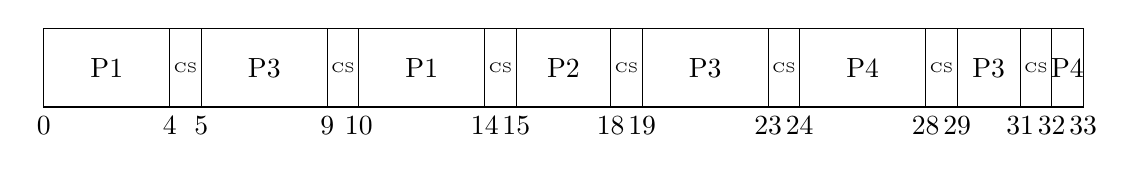
\begin{tikzpicture}[x=0.4cm, y=1cm]
    \draw (0,0) rectangle (4,1) node[midway] {P1};
    \draw (4,0) rectangle (5,1) node[midway, font=\tiny] {CS};
    \draw (5,0) rectangle (9,1) node[midway] {P3};
    \draw (9,0) rectangle (10,1) node[midway, font=\tiny] {CS};
    \draw (10,0) rectangle (14,1) node[midway] {P1};
    \draw (14,0) rectangle (15,1) node[midway, font=\tiny] {CS};
    \draw (15,0) rectangle (18,1) node[midway] {P2};
    \draw (18,0) rectangle (19,1) node[midway, font=\tiny] {CS};
    \draw (19,0) rectangle (23,1) node[midway] {P3};
    \draw (23,0) rectangle (24,1) node[midway, font=\tiny] {CS};
    \draw (24,0) rectangle (28,1) node[midway] {P4};
    \draw (28,0) rectangle (29,1) node[midway, font=\tiny] {CS};
    \draw (29,0) rectangle (31,1) node[midway] {P3};
    \draw (31,0) rectangle (32,1) node[midway, font=\tiny] {CS};
    \draw (32,0) rectangle (33,1) node[midway] {P4};
    
    \node[below] at (0,0) {0};
    \node[below] at (4,0) {4};
    \node[below] at (5,0) {5};
    \node[below] at (9,0) {9};
    \node[below] at (10,0) {10};
    \node[below] at (14,0) {14};
    \node[below] at (15,0) {15};
    \node[below] at (18,0) {18};
    \node[below] at (19,0) {19};
    \node[below] at (23,0) {23};
    \node[below] at (24,0) {24};
    \node[below] at (28,0) {28};
    \node[below] at (29,0) {29};
    \node[below] at (31,0) {31};
    \node[below] at (32,0) {32};
    \node[below] at (33,0) {33};
\end{tikzpicture}
\captionof{figure}{Gantt Chart (Round Robin)}
\end{center}
\textit{Note: The exact timeline may vary slightly depending on interpretation of CS handling, assuming CS happens after process switch.}

\textbf{Calculations:}

\begin{center}
\captionof{table}{Calculations}
\begin{tabulary}{\linewidth}{|L|L|L|L|}
\hline
\textbf{Process} & \textbf{Completion} & \textbf{Turnaround} & \textbf{Waiting} \\ \hline
P1 & 14 & 14 - 0 = 14 & 14 - 8 = 6 \\ \hline
P2 & 18 & 18 - 3 = 15 & 15 - 3 = 12 \\ \hline
P3 & 31 & 31 - 1 = 30 & 30 - 10 = 20 \\ \hline
P4 & 33 & 33 - 4 = 29 & 29 - 5 = 24 \\ \hline
\end{tabulary}
\end{center}

\textbf{Average Waiting Time} = $(6 + 12 + 20 + 24) / 4 = 15.5$ ms \\
\textbf{Average Turnaround Time} = $(14 + 15 + 30 + 29) / 4 = 22$ ms

\textbf{Key Features:}
\begin{itemize}
    \item \keyword{Fair Scheduling}: Each process gets equal CPU time
    \item \keyword{Preemptive}: Running process is interrupted after quantum expires
    \item \keyword{Context Switching}: Overhead included in calculations
\end{itemize}
\end{solutionbox}

\begin{mnemonicbox}
\mnemonic{FPC - Fair, Preemptive, Context switching overhead}
\end{mnemonicbox}

\questionmarks{2(a) OR}{3}{Differentiate: CPU bound process v/s I/O bound process.}

\begin{solutionbox}
\textbf{Answer}:

\begin{center}
\captionof{table}{CPU Bound vs I/O Bound}
\begin{tabulary}{\linewidth}{|L|L|L|}
\hline
\textbf{Aspect} & \textbf{CPU Bound Process} & \textbf{I/O Bound Process} \\ \hline
Primary Activity & Intensive calculations & Frequent I/O operations \\ \hline
CPU Usage & High CPU utilization & Low CPU utilization \\ \hline
Burst Time & Long CPU bursts & Short CPU bursts \\ \hline
Waiting Time & Less I/O waiting & More I/O waiting \\ \hline
Examples & Mathematical calculations & File operations, database queries \\ \hline
\end{tabulary}
\end{center}

\textbf{Key Differences:}
\begin{itemize}
    \item \keyword{Resource Consumption}: CPU-bound uses more processor, I/O-bound uses more input/output
    \item \keyword{Performance Impact}: CPU-bound affected by processor speed, I/O-bound by storage speed
    \item \keyword{Scheduling Priority}: Different algorithms favor each type differently
\end{itemize}
\end{solutionbox}

\begin{mnemonicbox}
\mnemonic{CIR - CPU intensive, I/O intensive, Resource usage differs}
\end{mnemonicbox}

\questionmarks{2(b) OR}{4}{What is a deadlock? Explain the necessary conditions for a deadlock to occur.}

\begin{solutionbox}
\textbf{Answer}:

\textbf{Deadlock} is a situation where two or more processes are permanently blocked, each waiting for resources held by others.

\textbf{Necessary Conditions (Coffman Conditions):}
\begin{center}
\captionof{table}{Coffman Conditions}
\begin{tabulary}{\linewidth}{|L|L|}
\hline
\textbf{Condition} & \textbf{Description} \\ \hline
Mutual Exclusion & Resources cannot be shared simultaneously \\ \hline
Hold and Wait & Process holds resources while waiting for others \\ \hline
No Preemption & Resources cannot be forcibly taken from processes \\ \hline
Circular Wait & Circular chain of processes waiting for resources \\ \hline
\end{tabulary}
\end{center}

\textbf{Example Scenario:}
\begin{center}
\begin{tikzpicture}[node distance=2cm, auto]
    \node [gtu state] (pa) {Process A};
    \node [gtu state, right=3cm of pa] (pb) {Process B};
    \node [gtu block, below=1.5cm of pa, minimum height=1cm] (r2) {Resource 2};
    \node [gtu block, above=1.5cm of pb, minimum height=1cm] (r1) {Resource 1};

    \draw [gtu arrow] (pa) -- node[left] {Holds} (r1);
    \draw [gtu arrow] (r1) -- node[above] {Waits} (pb);
    \draw [gtu arrow] (pb) -- node[right] {Holds} (r2);
    \draw [gtu arrow] (r2) -- node[below] {Waits} (pa);
\end{tikzpicture}
\captionof{figure}{Deadlock Scenario}
\end{center}
\end{solutionbox}

\begin{mnemonicbox}
\mnemonic{MHNC - Mutual exclusion, Hold-wait, No preemption, Circular wait}
\end{mnemonicbox}

\questionmarks{2(c) OR}{7}{Describe the FCFS algorithm. Calculate the average waiting time and average turn-around time along with Gantt chart for the given data.}

\begin{solutionbox}
\textbf{Answer}:

\textbf{First Come First Serve (FCFS) Algorithm:}
FCFS is a non-preemptive scheduling algorithm where processes are executed in arrival order.

\textbf{Given Data:}
\begin{center}
\captionof{table}{Process Data}
\begin{tabulary}{\linewidth}{|L|L|L|}
\hline
\textbf{Process} & \textbf{Arrival Time} & \textbf{Burst Time} \\ \hline
P1 & 0 & 7 \\ \hline
P2 & 3 & 6 \\ \hline
P3 & 5 & 9 \\ \hline
P4 & 6 & 4 \\ \hline
\end{tabulary}
\end{center}

\textbf{Gantt Chart:}
\begin{center}
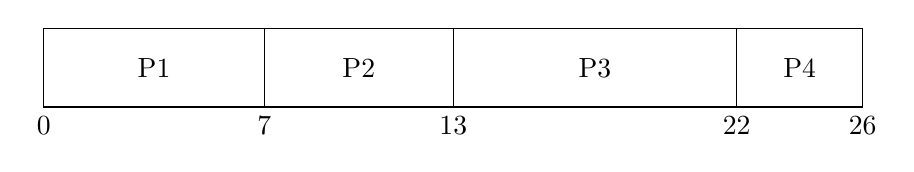
\begin{tikzpicture}[x=0.4cm, y=1cm]
    \draw (0,0) rectangle (7,1) node[midway] {P1};
    \draw (7,0) rectangle (13,1) node[midway] {P2};
    \draw (13,0) rectangle (22,1) node[midway] {P3};
    \draw (22,0) rectangle (26,1) node[midway] {P4};
    
    \node[below] at (0,0) {0};
    \node[below] at (7,0) {7};
    \node[below] at (13,0) {13};
    \node[below] at (22,0) {22};
    \node[below] at (26,0) {26};
\end{tikzpicture}
\captionof{figure}{Gantt Chart (FCFS)}
\end{center}

\textbf{Calculations:}

\begin{center}
\captionof{table}{FCFS Calculations}
\begin{tabulary}{\linewidth}{|L|L|L|}
\hline
\textbf{Process} & \textbf{Turnaround (CT-AT)} & \textbf{Waiting (TAT-BT)} \\ \hline
P1 & $7-0 = 7$ & $7-7 = 0$ \\ \hline
P2 & $13-3 = 10$ & $10-6 = 4$ \\ \hline
P3 & $22-5 = 17$ & $17-9 = 8$ \\ \hline
P4 & $26-6 = 20$ & $20-4 = 16$ \\ \hline
\end{tabulary}
\end{center}

\textbf{Avg Waiting Time} = $(0 + 4 + 8 + 16) / 4 = 7$ ms \\
\textbf{Avg Turnaround Time} = $(7 + 10 + 17 + 20) / 4 = 13.5$ ms

\textbf{Characteristics:}
\begin{itemize}
    \item \keyword{Simple Implementation}: Easy to understand and implement
    \item \keyword{Non-preemptive}: Once started, process runs to completion
    \item \keyword{Convoy Effect}: Short processes wait for long processes
\end{itemize}
\end{solutionbox}

\begin{mnemonicbox}
\mnemonic{SNC - Simple, Non-preemptive, Convoy effect possible}
\end{mnemonicbox}

\questionmarks{3(a)}{3}{Explain single-level directory structure.}

\begin{solutionbox}
\textbf{Answer}:

Single-level directory structure is the simplest file organization where all files are stored in one directory.

\begin{center}
\begin{tikzpicture}[node distance=1.5cm]
    \node [gtu block, minimum width=8cm] (root) {Root Directory};
    
    \node [gtu block, below=1cm of root, xshift=-3cm] (f1) {file1.txt};
    \node [gtu block, right=0.3cm of f1] (f2) {prog.exe};
    \node [gtu block, right=0.3cm of f2] (f3) {data.dat};
    \node [gtu block, right=0.3cm of f3] (f4) {img.jpg};
    
    \draw [gtu arrow] (root) -- (f1);
    \draw [gtu arrow] (root) -- (f2);
    \draw [gtu arrow] (root) -- (f3);
    \draw [gtu arrow] (root) -- (f4);
\end{tikzpicture}
\captionof{figure}{Single-level Directory}
\end{center}

\textbf{Characteristics:}
\begin{itemize}
    \item \keyword{Simple Structure}: All files in one location
    \item \keyword{Unique Names}: Each file must have unique name
    \item \keyword{No Organization}: No grouping or categorization possible
\end{itemize}

\textbf{Limitations:}
\begin{itemize}
    \item Name collision when multiple users create files with same names
    \item Difficult to organize large number of files
    \item No privacy or access control between users
\end{itemize}
\end{solutionbox}

\begin{mnemonicbox}
\mnemonic{SUN - Simple, Unique names, No organization}
\end{mnemonicbox}

\questionmarks{3(b)}{4}{Explain the different file attributes.}

\begin{solutionbox}
\textbf{Answer}:

File attributes are metadata that provide information about files stored in the file system.

\begin{center}
\captionof{table}{File Attributes}
\begin{tabulary}{\linewidth}{|L|L|}
\hline
\textbf{Attribute} & \textbf{Description} \\ \hline
Name & Human-readable file identifier \\ \hline
Type & File format (executable, text, image) \\ \hline
Size & Current file size in bytes \\ \hline
Location & Physical address on storage device \\ \hline
Protection & Access permissions (read, write, execute) \\ \hline
Time stamps & Creation, modification, access times \\ \hline
Owner & User who created the file \\ \hline
\end{tabulary}
\end{center}

\textbf{Common File Attributes:}
\begin{itemize}
    \item \keyword{Identifier}: Unique number for file system reference
    \item \keyword{Access Control}: User permissions and group access rights
\end{itemize}

\textbf{Storage Location:} File attributes are typically stored in directory entries or file allocation tables.
\end{solutionbox}

\begin{mnemonicbox}
\mnemonic{NTSLPTO - Name, Type, Size, Location, Protection, Time, Owner}
\end{mnemonicbox}

\questionmarks{3(c)}{7}{List the different file allocation methods and explain contiguous allocation with necessary diagram.}

\begin{solutionbox}
\textbf{Answer}:

\textbf{File Allocation Methods:}
\begin{itemize}
    \item \keyword{Contiguous}: Files stored in consecutive blocks
    \item \keyword{Linked}: Files stored using linked list of blocks
    \item \keyword{Indexed}: Uses index block to point to data blocks
\end{itemize}

\textbf{Contiguous Allocation:}
In contiguous allocation, each file occupies a set of contiguous blocks on the disk.

\begin{center}
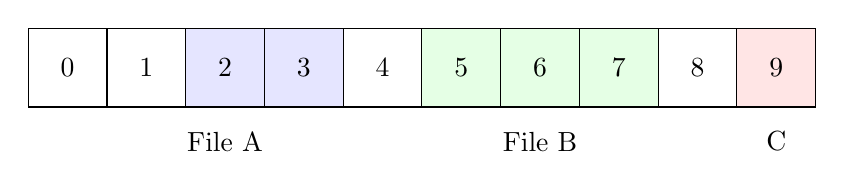
\begin{tikzpicture}[node distance=0cm, outer sep=0pt]
    \node [rectangle, draw, minimum width=1cm, minimum height=1cm] (b0) {0};
    \node [rectangle, draw, minimum width=1cm, minimum height=1cm, right=of b0] (b1) {1};
    \node [rectangle, draw, minimum width=1cm, minimum height=1cm, right=of b1, fill=blue!10] (b2) {2};
    \node [rectangle, draw, minimum width=1cm, minimum height=1cm, right=of b2, fill=blue!10] (b3) {3};
    \node [rectangle, draw, minimum width=1cm, minimum height=1cm, right=of b3] (b4) {4};
    \node [rectangle, draw, minimum width=1cm, minimum height=1cm, right=of b4, fill=green!10] (b5) {5};
    \node [rectangle, draw, minimum width=1cm, minimum height=1cm, right=of b5, fill=green!10] (b6) {6};
    \node [rectangle, draw, minimum width=1cm, minimum height=1cm, right=of b6, fill=green!10] (b7) {7};
    \node [rectangle, draw, minimum width=1cm, minimum height=1cm, right=of b7] (b8) {8};
    \node [rectangle, draw, minimum width=1cm, minimum height=1cm, right=of b8, fill=red!10] (b9) {9};
    
    \node [below=0.2cm of b2] {File A};
    \node [below=0.2cm of b6] {File B};
    \node [below=0.2cm of b9] {C};
\end{tikzpicture}

\vspace{0.5cm}

\captionof{table}{Directory Table}
\begin{tabular}{|c|c|c|}
\hline
\textbf{Filename} & \textbf{Start} & \textbf{Length} \\ \hline
File A & 2 & 2 \\ \hline
File B & 5 & 3 \\ \hline
File C & 9 & 1 \\ \hline
\end{tabular}
\end{center}

\textbf{Advantages:}
\begin{itemize}
    \item \keyword{Fast Access}: Direct calculation of block addresses
    \item \keyword{Minimal Seek Time}: Consecutive blocks reduce head movement
\end{itemize}

\textbf{Disadvantages:}
\begin{itemize}
    \item \keyword{External Fragmentation}: Unused spaces between files
    \item \keyword{File Size Limitation}: Difficult to extend files
\end{itemize}
\end{solutionbox}

\begin{mnemonicbox}
\mnemonic{FMS vs EFC - Fast access, Minimal seek, Simple vs External fragmentation, File size limits, Compaction needed}
\end{mnemonicbox}

\questionmarks{3(a) OR}{3}{Explain the different types of Linux file systems in brief.}

\begin{solutionbox}
\textbf{Answer}:

\begin{center}
\captionof{table}{Linux File Systems}
\begin{tabulary}{\linewidth}{|L|L|}
\hline
\textbf{File System} & \textbf{Description} \\ \hline
ext2 & Second extended filesystem, no journaling \\ \hline
ext3 & Third extended filesystem with journaling \\ \hline
ext4 & Fourth extended filesystem, improved performance \\ \hline
XFS & High-performance 64-bit journaling filesystem \\ \hline
Btrfs & B-tree filesystem with advanced features \\ \hline
ZFS & Copy-on-write filesystem with data integrity \\ \hline
\end{tabulary}
\end{center}

\textbf{Key Features:}
\begin{itemize}
    \item \keyword{Journaling}: ext3, ext4, XFS provide crash recovery
    \item \keyword{Performance}: ext4, XFS optimized for large files
    \item \keyword{Advanced Features}: Btrfs, ZFS offer snapshots and compression
\end{itemize}
\end{solutionbox}

\begin{mnemonicbox}
\mnemonic{EEXBZ - ext2/3/4, XFS, Btrfs, ZFS options}
\end{mnemonicbox}

\questionmarks{3(b) OR}{4}{Explain the different file operations.}

\begin{solutionbox}
\textbf{Answer}:

\begin{center}
\captionof{table}{File Operations}
\begin{tabulary}{\linewidth}{|L|L|}
\hline
\textbf{Operation} & \textbf{Description} \\ \hline
Create & Make new file with specified name and attributes \\ \hline
Open & Prepare file for reading/writing operations \\ \hline
Read & Retrieve data from file at current position \\ \hline
Write & Store data to file at current position \\ \hline
Seek & Move file pointer to specific position \\ \hline
Close & Release file resources and update metadata \\ \hline
Delete & Remove file and deallocate storage space \\ \hline
\end{tabulary}
\end{center}

\textbf{File Operation Sequence:}

\begin{center}
\begin{tikzpicture}[node distance=1.5cm, auto]
    \node [gtu state] (create) {Create File};
    \node [gtu state, right=of create] (open) {Open File};
    \node [gtu state, right=of open] (rw) {Read/Write};
    \node [gtu state, below=of rw] (seek) {Seek};
    \node [gtu state, right=of rw] (close) {Close File};
    \node [gtu state, right=of close] (del) {Delete};

    \path [gtu arrow] (create) -- (open);
    \path [gtu arrow] (open) -- (rw);
    \path [gtu arrow] (rw) -- (close);
    \path [gtu arrow] (close) -- (del);
    \path [gtu arrow] (rw) edge [bend right] (seek);
    \path [gtu arrow] (seek) edge [bend right] (rw);
\end{tikzpicture}
\captionof{figure}{File Operation Sequence}
\end{center}
\end{solutionbox}

\begin{mnemonicbox}
\mnemonic{CORWSCD - Create, Open, Read, Write, Seek, Close, Delete}
\end{mnemonicbox}

\questionmarks{3(c) OR}{7}{List the different file allocation methods and explain indexed allocation with necessary diagram.}

\begin{solutionbox}
\textbf{Answer}:

\textbf{Indexed Allocation:}
In indexed allocation, each file has an index block containing pointers to data blocks.

\begin{center}
\begin{tikzpicture}[node distance=1.5cm]
    \node [rectangle, draw, fill=yellow!10, inner sep=0pt] (index) {\begin{tabular}{c}\textbf{Index Block}\\ \hline 2\\5\\8\\9\end{tabular}};
    \node [gtu block, right=of index, yshift=1.5cm] (b2) {Block 2};
    \node [gtu block, right=of index, yshift=0.5cm] (b5) {Block 5};
    \node [gtu block, right=of index, yshift=-0.5cm] (b8) {Block 8};
    \node [gtu block, right=of index, yshift=-1.5cm] (b9) {Block 9};
    
    \draw [->] (index.east) -- (b2.west);
    \draw [->] (index.east) -- (b5.west);
    \draw [->] (index.east) -- (b8.west);
    \draw [->] (index.east) -- (b9.west);
\end{tikzpicture}
\captionof{figure}{Indexed Allocation}
\end{center}

\textbf{Advantages:}
\begin{itemize}
    \item \keyword{No External Fragmentation}: Blocks can be anywhere on disk
    \item \keyword{Dynamic File Size}: Easy to extend files
    \item \keyword{Fast Random Access}: Direct access to any block
\end{itemize}

\textbf{Disadvantages:}
\begin{itemize}
    \item \keyword{Index Block Overhead}: Extra space for pointers
    \item \keyword{Multiple Disk Access}: Two accesses needed (index + data)
\end{itemize}
\end{solutionbox}

\begin{mnemonicbox}
\mnemonic{NDF vs IMI - No fragmentation, Dynamic size, Fast access vs Index overhead, Multiple access}
\end{mnemonicbox}

\questionmarks{4(a)}{3}{Define System threats and explain its types.}

\begin{solutionbox}
\textbf{Answer}:

\textbf{System Threats} are malicious attempts to disrupt or damage computer system operations, steal information, or gain unauthorized access.

\begin{center}
\captionof{table}{System Threats}
\begin{tabulary}{\linewidth}{|L|L|}
\hline
\textbf{Threat Type} & \textbf{Description} \\ \hline
Worms & Self-replicating programs that spread across networks \\ \hline
Viruses & Malicious code that attaches to other programs \\ \hline
Trojan Horses & Legitimate-looking programs with hidden malicious functions \\ \hline
Denial of Service & Attacks that overwhelm system resources \\ \hline
Port Scanning & Unauthorized probing of network services \\ \hline
\end{tabulary}
\end{center}

\textbf{Impact:} System threats can lead to data loss, system downtime, privacy breaches, and financial damage.
\end{solutionbox}

\begin{mnemonicbox}
\mnemonic{WVTDP - Worms, Viruses, Trojans, DoS, Port scanning}
\end{mnemonicbox}

\questionmarks{4(b)}{4}{Differentiate: User Authentication v/s User Authorization.}

\begin{solutionbox}
\textbf{Answer}:

\begin{center}
\captionof{table}{Authentication vs Authorization}
\begin{tabulary}{\linewidth}{|L|L|L|}
\hline
\textbf{Aspect} & \textbf{User Authentication} & \textbf{User Authorization} \\ \hline
Purpose & Verify user identity & Determine user permissions \\ \hline
When & Before system access & After authentication \\ \hline
Methods & Passwords, biometrics & Access control lists, roles \\ \hline
Question & "Who are you?" & "What can you do?" \\ \hline
Process & One-time at login & Continuous during session \\ \hline
\end{tabulary}
\end{center}

\textbf{Relationship:} Authentication must occur before authorization.
\end{solutionbox}

\begin{mnemonicbox}
\mnemonic{WHO vs WHAT - Authentication asks WHO, Authorization determines WHAT}
\end{mnemonicbox}

\questionmarks{4(c)}{7}{Discuss various operating system security policies and procedures.}

\begin{solutionbox}
\textbf{Answer}:

\textbf{Security Policies:}
\begin{itemize}
    \item \keyword{Access Control}: Defines who can access what resources
    \item \keyword{Password Policy}: Rules for password creation and management
    \item \keyword{Audit Policy}: Logging and monitoring of system activities
    \item \keyword{Update Policy}: Regular security patches and updates
    \item \keyword{Data Classification}: Categorizing data by sensitivity levels
\end{itemize}

\textbf{System Monitoring Flow:}
\begin{center}
\begin{tikzpicture}[node distance=1.5cm, auto]
    \node [gtu state] (log) {Log Collection};
    \node [gtu state, right=of log] (ana) {Analysis};
    \node [gtu state, right=of ana] (det) {Detection};
    \node [gtu state, below=of det] (alert) {Alert};
    \node [gtu state, left=of alert] (resp) {Response};

    \path [gtu arrow] (log) -- (ana);
    \path [gtu arrow] (ana) -- (det);
    \path [gtu arrow] (det) -- (alert);
    \path [gtu arrow] (alert) -- (resp);
\end{tikzpicture}
\captionof{figure}{Security Monitoring}
\end{center}

\textbf{Security Procedures:}
\begin{itemize}
    \item \keyword{User Account Management}: Review accounts, revoke access
    \item \keyword{Incident Response}: Detection, containment, recovery
    \item \keyword{Backup and Recovery}: Regular backups, disaster planning
\end{itemize}
\end{solutionbox}

\begin{mnemonicbox}
\mnemonic{AAPUD + UMSIR - Policies + Procedures}
\end{mnemonicbox}

\questionmarks{4(a) OR}{3}{Define Program threats and explain its types.}

\begin{solutionbox}
\textbf{Answer}:

\textbf{Program Threats} are malicious software designed to disrupt, damage, or gain unauthorized access to computer programs and data.

\begin{center}
\captionof{table}{Program Threats}
\begin{tabulary}{\linewidth}{|L|L|}
\hline
\textbf{Threat Type} & \textbf{Description} \\ \hline
Malware & Malicious software including viruses, worms \\ \hline
Spyware & Programs that secretly monitor user activities \\ \hline
Adware & Unwanted advertising software \\ \hline
Ransomware & Encrypts data and demands payment \\ \hline
Rootkits & Hide malicious activities from detection \\ \hline
\end{tabulary}
\end{center}
\end{solutionbox}

\begin{mnemonicbox}
\mnemonic{MSARR - Malware, Spyware, Adware, Ransomware, Rootkits}
\end{mnemonicbox}

\questionmarks{4(b) OR}{4}{Explain the protection domain with a suitable example.}

\begin{solutionbox}
\textbf{Answer}:

\textbf{Protection Domain} is a set of objects and access rights that define what resources a process can access.

\textbf{Domain Structure Example:}

\begin{center}
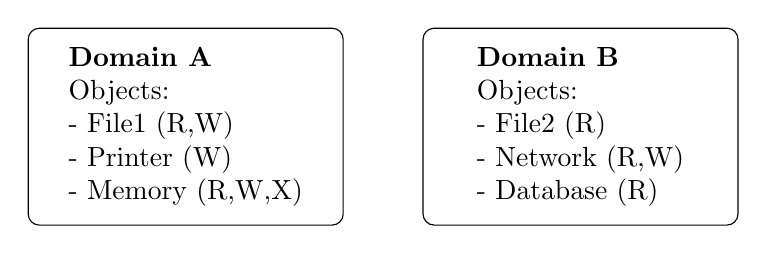
\begin{tikzpicture}[node distance=1cm]
    \node [rectangle, draw, rounded corners, minimum width=4cm, minimum height=2.5cm, align=left] (da) {\textbf{Domain A}\\ Objects:\\ - File1 (R,W)\\ - Printer (W)\\ - Memory (R,W,X)};
    
    \node [rectangle, draw, rounded corners, minimum width=4cm, minimum height=2.5cm, align=left, right=1cm of da] (db) {\textbf{Domain B}\\ Objects:\\ - File2 (R)\\ - Network (R,W)\\ - Database (R)};
\end{tikzpicture}
\captionof{figure}{Protection Domains}
\end{center}

\textbf{Benefits:}
\begin{itemize}
    \item \keyword{Isolation}: Prevents unauthorized access
    \item \keyword{Flexibility}: Controlled resource sharing
    \item \keyword{Security}: Least privilege principle
\end{itemize}
\end{solutionbox}

\begin{mnemonicbox}
\mnemonic{OAS - Objects, Access rights, Subjects define domains}
\end{mnemonicbox}

\questionmarks{4(c) OR}{7}{Explain Access Control List in detail.}

\begin{solutionbox}
\textbf{Answer}:

\textbf{Access Control List (ACL)} specifies which users or processes are granted access to objects.

\textbf{ACL Implementation:}
\begin{center}
\begin{tabular}{|l|l|}
\hline
\multicolumn{2}{|c|}{\textbf{File: /home/project/report.txt}} \\ \hline
\textbf{User} & \textbf{Permissions} \\ \hline
alice & read, write \\ \hline
bob & read \\ \hline
admin & read, write, delete \\ \hline
group:dev & read, write \\ \hline
\end{tabular}
\captionof{table}{ACL Example}
\end{center}

\textbf{Advantages:}
\begin{itemize}
    \item \keyword{Granular Control}: Fine-grained permission management
    \item \keyword{Audit Trail}: Clear record of who has access
\end{itemize}

\textbf{Disadvantages:}
\begin{itemize}
    \item \keyword{Performance Overhead}: Must check ACL for each access
    \item \keyword{Complexity}: Difficult to manage for many users/objects
\end{itemize}
\end{solutionbox}

\begin{mnemonicbox}
\mnemonic{SOA + GDSC - Subject, Object, Access + Granular, Distributed, Centralized}
\end{mnemonicbox}

\questionmarks{5(a)}{3}{Explain the following commands: (i) man (ii) cd (iii) ls}

\begin{solutionbox}
\textbf{Answer}:

\begin{center}
\captionof{table}{Basic Commands}
\begin{tabulary}{\linewidth}{|L|L|L|}
\hline
\textbf{Command} & \textbf{Purpose} & \textbf{Syntax} \\ \hline
man & Display manual pages & \code{man [cmd]} \\ \hline
cd & Change directory & \code{cd [dir]} \\ \hline
ls & List directory contents & \code{ls [opts] [dir]} \\ \hline
\end{tabulary}
\end{center}

\textbf{Details:}
\begin{itemize}
    \item \keyword{man}: Shows documentation (e.g., \code{man ls})
    \item \keyword{cd}: Navigates filesystem (e.g., \code{cd /home}, \code{cd ..})
    \item \keyword{ls}: Lists files (e.g., \code{ls -la} for hidden files)
\end{itemize}
\end{solutionbox}

\begin{mnemonicbox}
\mnemonic{MCD - Manual pages, Change directory, Directory listing}
\end{mnemonicbox}

\questionmarks{5(b)}{4}{Write a shell script to find maximum number among three numbers.}

\begin{solutionbox}
\begin{lstlisting}[language=bash, caption={Maximum of 3 Numbers}]
#!/bin/bash
# Script to find maximum among three numbers

echo "Enter three numbers:"
read -p "First number: " num1
read -p "Second number: " num2  
read -p "Third number: " num3

if [ $num1 -gt $num2 ]; then
    if [ $num1 -gt $num3 ]; then
        max=$num1
    else
        max=$num3
    fi
else
    if [ $num2 -gt $num3 ]; then
        max=$num2
    else
        max=$num3
    fi
fi

echo "Maximum number is: $max"
\end{lstlisting}
\end{solutionbox}

\begin{mnemonicbox}
\mnemonic{ICD - Input, Compare, Display result}
\end{mnemonicbox}

\questionmarks{5(c)}{7}{Write a shell script to find the sum of all the individual digits in a given 5-digit number.}

\begin{solutionbox}
\begin{lstlisting}[language=bash, caption={Sum of Digits}]
#!/bin/bash
# Script to find sum of digits in a 5-digit number

echo "Enter a 5-digit number:"
read number

# Validate input
if [ ${#number} -ne 5 ] || ! [[ $number =~ ^[0-9]+$ ]]; then
    echo "Error: Please enter exactly 5 digits"
    exit 1
fi

sum=0
temp=$number

# Extract and sum each digit
while [ $temp -gt 0 ]; do
    digit=$((temp % 10))    # Get last digit
    sum=$((sum + digit))    # Add to sum
    temp=$((temp / 10))     # Remove last digit
done

echo "Number: $number"
echo "Sum of digits: $sum"
\end{lstlisting}
\end{solutionbox}

\begin{mnemonicbox}
\mnemonic{VEDS - Validate, Extract, Display, Sum digits}
\end{mnemonicbox}

\questionmarks{5(a) OR}{3}{Explain the following commands: (i) date (ii) top (iii) cmp}

\begin{solutionbox}
\textbf{Answer}:

\begin{center}
\captionof{table}{More Commands}
\begin{tabulary}{\linewidth}{|L|L|L|}
\hline
\textbf{Cmd} & \textbf{Purpose} & \textbf{Example} \\ \hline
date & Display/set system date & \code{date +\%F} \\ \hline
top & Real-time process view & \code{top} \\ \hline
cmp & Byte-by-byte file compare & \code{cmp f1 f2} \\ \hline
\end{tabulary}
\end{center}
\end{solutionbox}

\begin{mnemonicbox}
\mnemonic{DTC - Date/time, Task monitor, Compare files}
\end{mnemonicbox}

\questionmarks{5(b) OR}{4}{Explain the installation steps of Linux.}

\begin{solutionbox}
\textbf{Answer}:

\textbf{Installation Process:}

\begin{center}
\begin{tikzpicture}[node distance=0.8cm, auto]
    \node [gtu state] (iso) {Download ISO};
    \node [gtu state, right=of iso] (media) {Create Media};
    \node [gtu state, right=of media] (boot) {Boot};
    \node [gtu state, below=of iso] (part) {Partition};
    \node [gtu state, right=of part] (user) {User Setup};
    \node [gtu state, right=of user] (install) {Install};
    
    \path [gtu arrow] (iso) -- (media);
    \path [gtu arrow] (media) -- (boot);
    \path [gtu arrow] (boot) -- (part);
    \path [gtu arrow] (part) -- (user);
    \path [gtu arrow] (user) -- (install);
\end{tikzpicture}
\captionof{figure}{Installation Flow}
\end{center}

\textbf{Key Steps:}
\begin{enumerate}
    \item \keyword{Partitioning}: Configure disk space (root, home, swap)
    \item \keyword{Configuration}: Set timezone, keyboard, user accounts
    \item \keyword{Installation}: Copy system files and install bootloader
\end{enumerate}
\end{solutionbox}

\begin{mnemonicbox}
\mnemonic{DCBCPUPI - Download, Create, Boot, Choose, Partition, User, Package, Install}
\end{mnemonicbox}

\questionmarks{5(c) OR}{7}{Write a shell script to find sum and average of N numbers.}

\begin{solutionbox}
\begin{lstlisting}[language=bash, caption={Sum and Average of N Numbers}]
#!/bin/bash
# Script to find sum and average of N numbers

echo "How many numbers do you want to enter?"
read n

# Validate input
if ! [[ $n =~ ^[0-9]+$ ]] || [ $n -le 0 ]; then
    echo "Error: Please enter a positive integer"
    exit 1
fi

sum=0
echo "Enter $n numbers:"

# Read N numbers
for ((i=1; i<=n; i++)); do
    echo -n "Enter number $i: "
    read number
    # Simple accumulation
    sum=$(echo "$sum + $number" | bc -l)
done

# Calculate average
average=$(echo "scale=2; $sum / $n" | bc -l)

echo "Sum: $sum"
echo "Average: $average"
\end{lstlisting}
\end{solutionbox}

\begin{mnemonicbox}
\mnemonic{VLAD - Validate, Loop, Arithmetic, Display}
\end{mnemonicbox}

\end{document}
